\documentclass{article}
\usepackage[utf8]{inputenc}
\usepackage{hyperref}
\usepackage{float}
\usepackage{graphicx}
\usepackage[capitalize, nameinlink]{cleveref}   % Specify reference types (e.g. Table, Figure)
\usepackage{setspace}
\usepackage{svg}

% References
\usepackage[
    backend=biber,
    style=numeric,
]{biblatex}
\addbibresource{refs.bib}

\newcommand{\customcite}[1]{\citeauthor{#1} \cite{#1}}  % Cite author and reference


\begin{document}

% Based on https://www.overleaf.com/learn/latex/How_to_Write_a_Thesis_in_LaTeX_(Part_5)%3A_Customising_Your_Title_Page_and_Abstract
\begin{titlepage}
   \begin{center}
        
        \Large
        
        THE COOPER UNION \\
        FOR THE ADVANCEMENT OF SCIENCE AND ART\\
        ALBERT NERKEN SCHOOL OF ENGINEERING
        
        \vspace{4cm}
        \textbf{\LARGE \uppercase{Image Vectorization\\for Architecture}}
        
        \vspace{4cm}
        Jonathan Lam, Derek Lee, Victor Zhang\\
        
        \vspace{4cm}
        ECE395 Mid-year Report\\
        Professor Sam Keene\\
        December 2021
        
        \vfill
        
        \normalsize
   \end{center}
\end{titlepage}

\clearpage

\doublespacing
\tableofcontents
\clearpage

%%%%%%%%%%%%%%%%%%%%%%%%%%%%%%%%%%%%%%%%%%%%
\section{Abstract}

Architecture projects often involve both large structures and detailed components, and are often highly geometric. Digital architecture designs (i.e., created through the use of CAD) are often stored in a vector (shape-based) format for convenient editing. Raster (pixel-based) images, such as photographs, are not as easily used for these purposes, which largely diminishes their usability for the design process. Our project aims to develop a image vectorization method (i.e., a tool to convert from raster to vector format) specialized towards architecture images and explores the potential of vector-based images in the architecture design process and in machine learning preprocessing.

There are several general methods for image vectorization -- we propose a sampling-based vectorization method involving three steps. The image is sampled using a blue-noise sampling technique, which extracts the high frequency components in the image and filters out the less important pixels. The sampled point cloud is then simplified to reduce the number of vectors in the final drawing. Finally, the last step involves converting the point cloud to an efficient vector representation. This vector representation is saved as some vector image format, such as SVG.

%%%%%%%%%%%%%%%%%%%%%%%%%%%%%%%%%%%%%%%%%%%%
\clearpage
\section{Introduction}

%%%%%%%%%%%%%%%%%%%%%%%%%%%%%%%%%
\subsection{Goal}

Our project aims to provide an end-to-end image vectorization tool. Vectorization is the process of generating a vector image that is faithful to the input raster image. We aim to specialize in architectural images specifically, which should allow us to optimize our project for this use case. Architectural images are usually highly geometric, which should allow for an efficient vector representation. In theory, a highly geometric image should have a vector representation that is more efficient than the original image. Of course, with real images, the image will not be perfectly geometric. However, we are comfortable with information loss, as long as the main content of the image is preserved; we will develop a suitable loss metric to quantify the representation efficiency and error loss.

%%%%%%%%%%%%%%%%%%%%%%%%%%%%%%%%%
\subsection{Previous Works and Motivation}

Some of the first image vectorization tools implemented edge tracing, which works well for simple shapes, and especially in black-and-white (or similarly color-thresholded) images. However, architectural images are more complex and can have wide range of colors, rendering traditional methods ineffective. A new vectorization method is needed to work effectively for colored complex images and to generate vector representations that are easy to use for architects. 

%%%%%%%%%%%%%%%%%%%%%%%%%%%%%%%%%%%%%%%%%%%%% insert motivation for specializing in architecture

%%%%%%%%%%%%%%%%%%%%%%%%%%%%%%%%%
\subsection{Methods}

Multiple methods have been considered for this project, including traditional edge tracing, machine learning, and sampling. These methods are compared, and we determined that the sampling method is the most effective for our use case.  

%%%%%%%%%%%%%%%%%%%%%%%%%%%%%%%%%
\subsection{Potential Applications}

Our project can potentially be applied to the architecture design process, along with vector-based machine learning. One of the use cases we envision is to take a photo of an architectural design, use our project to process that image, and use the vector-based output to easily edit the image. Another potential use case is for vector-based machine learning. In computer vision, image data used as input is traditionally in raster format -- there is little research performed on how well deep learning performs on vector-based image inputs. We imagine that due to the efficiency of its representation, especially for highly-geometric shapes, we may be able to have more useful information in the deep learning model from the outset. In other words, a conversion to vector-based models, in which the shapes contain meaningful information about the image, may be useful as a machine learning preprocessing step.

%%%%%%%%%%%%%%%%%%%%%%%%%%%%%%%%%%%%%%%%%%%%
\clearpage
\section{Background}
%%%%%%%%%%%%%%%%%%%%%%%%%%%%%%%%%
\subsection{Raster Graphics}

Raster images are the simple matrix representation of an image. A raster image is conceptually a matrix of pixels, or a bitmap. Each pixel may contain multiple data points representing channels (colors). Historically, bitmaps have been the dominant representation for images due to their conceptual simplicity and the array-based display (and framebuffer) of modern screen technology. Much effort has been spent in enhancing the compression (e.g., lossy JPEG compression vs. lossless PNG compression) and analysis of raster images. Many image analysis methods depend on the grid-like representation of raster images, such as in the case of efficient parallel computation. Standardized raster images tend to have better support than vector graphics on older devices.

%%%%%%%%%%%%%%%%%%%%%%%%%%%%%%%%%
\subsection{Vector Graphics}

Vector graphics are not represented as pixels, but rather as a collection of parameterized geometric shapes. One of the immediate benefits is an efficient representation for purely geometric images, and the efficient and perfect scaling of continuous geometric objects. In order to display a vector image onto a pixel-based screen, the vector image first has to be rasterized, or rendered. Vector graphics are especially useful for web graphics and other highly geometric designs, such as maps, CAD, and typography. However, vector-based designs tend to be more inefficient for arbitrary image data (with high entropy), due to the relative complexity of shapes to pixels.

%%%%%%%%%%%%%%%%%%%%%%%%%%%%%%%%%
\subsection{Scalable Vector Graphics File Format}

Scalable Vector Graphics, or SVG, is a standard for vector graphics that uses the XML text format. All elements are represented using combinations of seven geometric shapes: Path, Rectangle, Circle, Ellipse, Line, Polyline, and Polygon. Since it is a textual format, it can be easily examined and manipulated by computers or by humans. The SVG standard is stable and supported by many applications, including PDF viewers and web browsers.

%%%%%%%%%%%%%%%%%%%%%%%%%%%%%%%%%
\subsection{Content Loss}

Content loss was introduced in \customcite{dumoulin2017learned}. The purpose of content loss is to quantify the difference in content between two images. Content loss was introduced as a loss function to train generative adversarial networks for style transfer.

The authors define the content loss between two images as the Euclidean distance between the high-level outputs of a trained classifier. This stems from a theory about deep convolutional neural networks: the early layers in a classifier are used to extract low-level features, such as edges, while the later layers of the classifier use the low-level features to create high-level features, such as an arm or a leg.

We tested the content loss metric on three images related to style transfer. The images were from \url{https://www.tensorflow.org/tutorials/generative/style_transfer}. 

\begin{figure}[H]
    \centering
    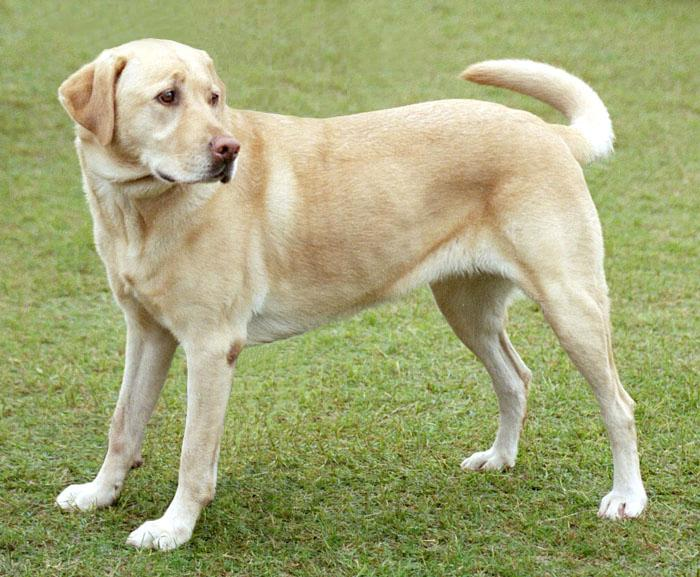
\includegraphics[width=\linewidth]{Figures/content_loss_images/lab1.jpg}
    \caption{\href{https://commons.wikimedia.org/wiki/File:YellowLabradorLooking_new.jpg}{Yellow Labrador Looking}, from Wikimedia Commons}
    \label{fig:lab_original}
\end{figure}

\begin{figure}[H]
    \centering
    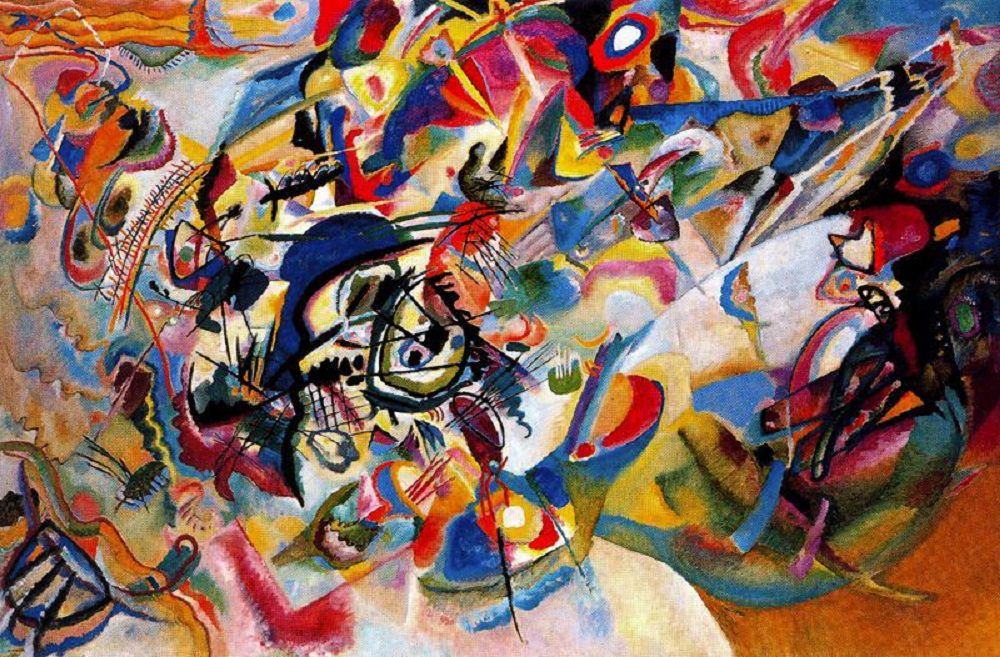
\includegraphics[width=\linewidth]{Figures/content_loss_images/lab2.jpg}
    \caption{Composition VII by Wassily Kandinsky}
    \label{fig:lab_style}
\end{figure}

\begin{figure}[H]
    \centering
    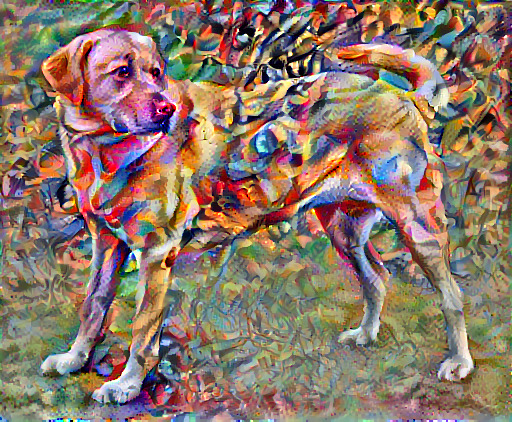
\includegraphics[width=\linewidth]{Figures/content_loss_images/lab3.jpg}
    \caption{Generated image produced with style transfer}
    \label{fig:lab_style_transfer}
\end{figure}

\cref{fig:lab_style_transfer} is generated using the content from \cref{fig:lab_original} and the style from \cref{fig:lab_style}. The content loss between \cref{fig:lab_original} and \cref{fig:lab_style_transfer} should be the lowest, compared to the content loss between \cref{fig:lab_original} and \cref{fig:lab_style}, because the two images have the same content but with different style. 


%%%%%%%%%%%%%%%%%%%%%%%%%%%%%%%%%%%%%%%%%%%%
\clearpage
\section{Related Work}
%%%%%%%%%%%%%%%%%%%%%%%%%%%%%%%%%
\subsection{Tracing Methods for Vectorization}

One of the successful earlier methods in image vectorization is called tracing, and at the time was synonymous with image vectorization. The general intuition behind this is that a raster image can be thought of as a collection of adjacent image patches, and we can vectorize an image by detecting edges of shapes.

\begin{figure}
    \centering
    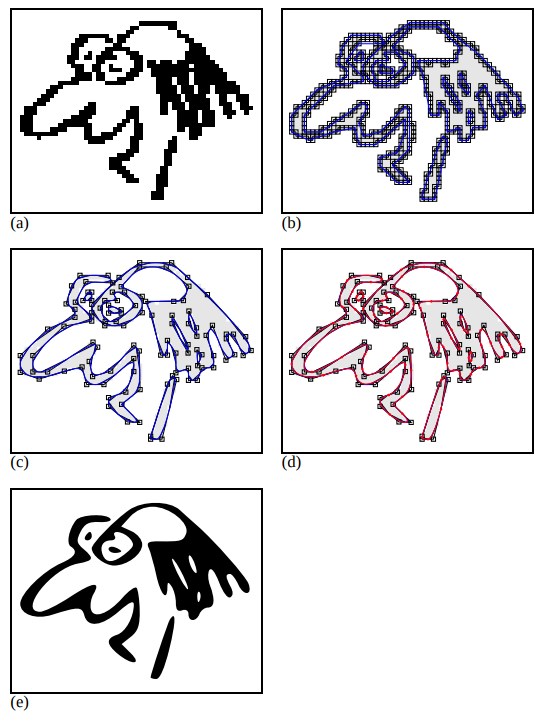
\includegraphics[width=\textwidth]{Figures/potrace.png}
    \caption{An illustration of the Potrace \cite{selinger2003potrace} vectorization process}
    \label{fig:potrace}
\end{figure}

A noteworthy implementation of image tracing is the Potrace algorithm \cite{selinger2003potrace}. As the name suggests, Potrace first attempts to convert a raster image into a series of polygonal paths via edge detection and straight-line detection, and then attempts to simplify (optimize) polygons by reducing path cardinalities and introducing Bezier curves. It employs many useful heuristics to improve image quality, such as removing speckles smaller than a given ``turd size'', detecting and smoothing corners, redundancy coding in the target format, scaling and rotating a small set of parameterized curves, and data quantization. An illustration of the stages of the Potrace algorithm is shown in \cref{fig:potrace}. The implementation of Potrace is open-source, and the program is highly configurable via command-line options.

This interpretation of vectorization is useful for simple raster images that are indeed a collection of adjacent shapes, such as map data, floor charts, typography, or charts. For such images, the Potrace algorithm is both reliable and efficient. While we do not use Potrace in our implementation, we may borrow some of its features related to curve optimization when simplifying the shapes (this is future work).

One of the drawbacks of tracing is that we can only trace edges on a binary thresholded image; if there aren't clearly defined edges, or if there are image gradients (as is often the case), it doesn't represent an image as well. Tracing can be applied to color images by thresholding the image by color or brightness level, and producing vector images for each thresholded layer, but this may seem choppy and low-quality. Tracing also does not recognize non-contiguous shapes (e.g., simple shapes that intersect other shapes), which can allow for more aggressive optimization and better object recognition. Machine learning approaches are better at recognizing this (citation).

%%%%%%%%%%%%%%%%%%%%%%%%%%%%%%%%%
\subsection{Machine Learning Approaches to Vectorization}

\begin{figure}[H]
    \centering
    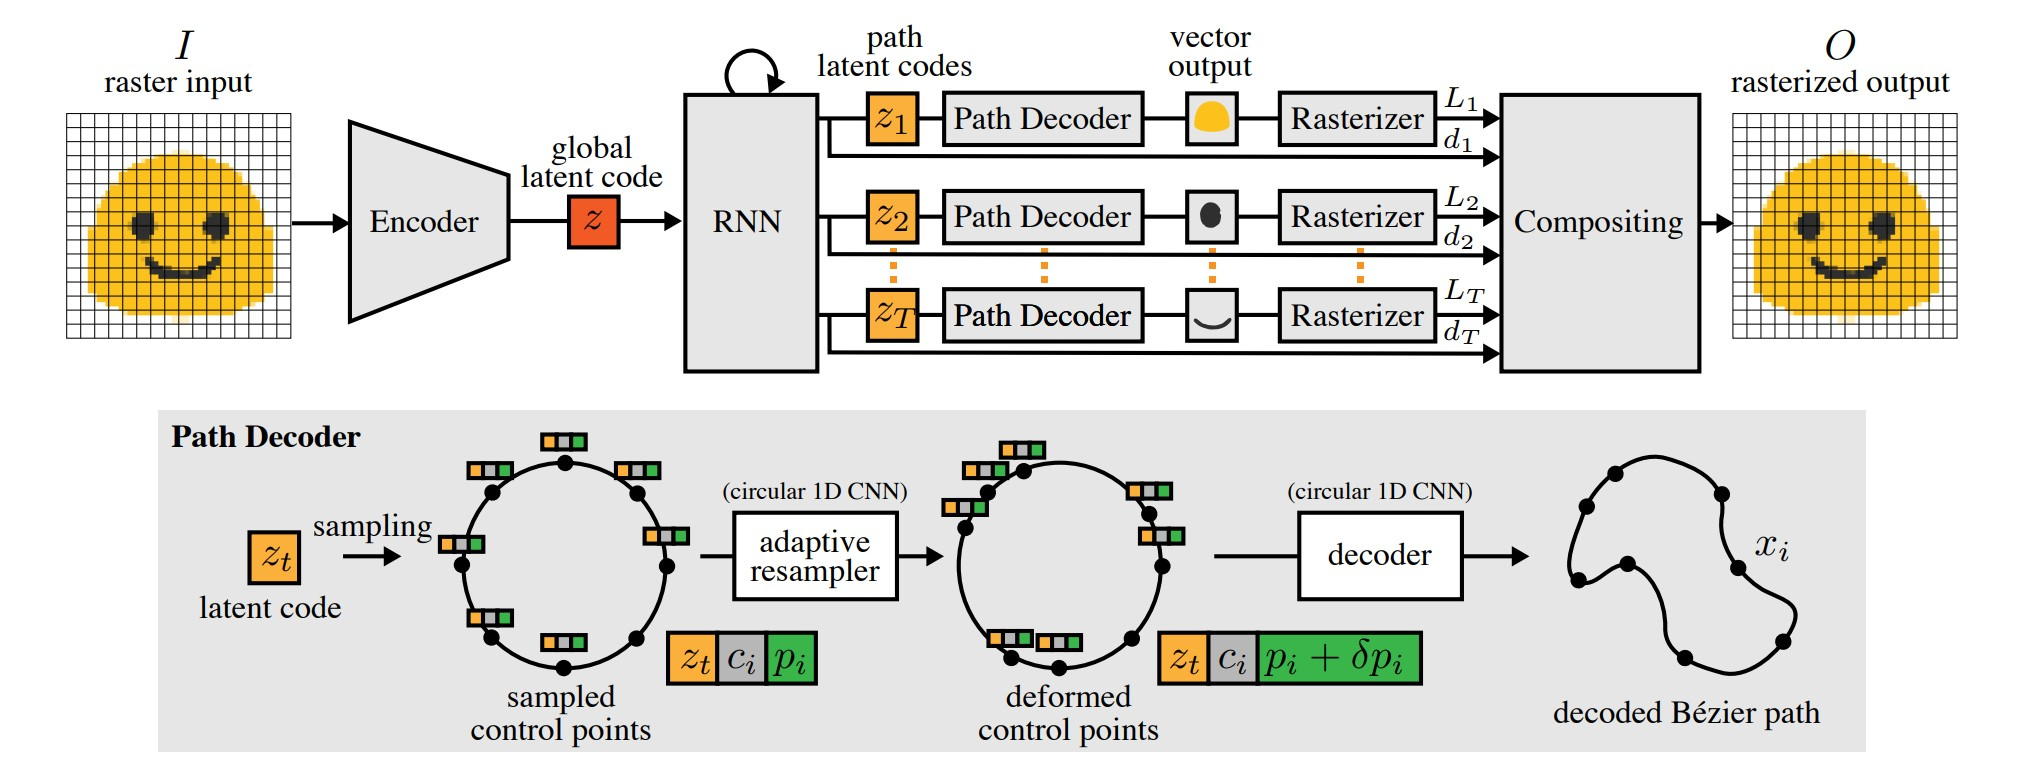
\includegraphics[width=\linewidth]{Figures/im2vec_architecture.jpg}
    \caption{Architecture overview for Im2Vec from \cite{reddy2021im2vec}}
\end{figure}

Im2Vec is an end-to-end deep neural network introduced by \customcite{reddy2021im2vec}. The model takes a raster image as input and outputs an SVG image. The raster image is first passed through an encoder. The encoded representation is then passed through a Recurrent Neural Network (RNN), specifically a bidirectional Long Short-Term Memory network (LSTM), to produce an arbitrary number outputs. Each output is passed through a path decoder, which produces a Bézier path. 

The path decoder uses continuous deformation of the unit circle to ensure each path is closed. The authors sample points on the unit circle and concatenate the output of the RNN to each of the sampled points. The authors next use 1D convolutions, equivalent to convolution around the perimeter of the circle, to determine how to deform the unit circle.

This model is trained by appending a differentiable rasterizer to the output. The rasterizer converts the vector output back to raster format and the resulting image can be compared to the original image to compute a loss. Since the rasterizer is differentiable, that loss can be backpropagated through the model. 

We explored using this model as part of our approach, but after looking through the codebase, we discovered that this would likely not work for our purposes. It appears that the authors hard-coded the number of shapes in the input raster image, along with the colors that each shape should be. We are looking to apply our model to various types of architectures, which will likely not be as well-defined as the emojis used in their experiments.

%%%%%%%%%%%%%%%%%%%%%%%%%%%%%%%%%
\subsection{Sampling Methods for Vectorization}

Sampling methods tackle the vectorization problem by stochastically approximating regions of the vector image. This allows us to achieve a reasonable performance and accuracy. Sampling methods may approximate edges less accurately than edge tracing, but they can overcome some of tracing's limitations, namely being limited to binary thresholding. Like tracing methods, it extends fairly well to more complicated images, while machine learning methods currently appear to be more limited to simple images.

%%%%%%%%%%%%%%%%% Move this citation to the appropriate place
An example procedure for image vectorization through sampling is shown in Zhao et al.'s work \customcite{zhao2013image}. The sampling method for vectorization is composed of 3 steps. The image is first convoluted with a Sobel differential operator to generate an ``importance matrix''. This represents the discontinuities or gradients in the original matrix; larger gradients may indicate regions with more detail. We then apply blue-noise sampling to the image using the importance matrix to determine sampling density around each pixel, with a larger gradient causing a higher sampling density. The sampled points are then triangulated, and the line segments of the triangles form the vector representation of the image. 

%%%%%%%%%%%%%%%%%%%%%%%%%%%%%%%%%
\subsection{Vector Image Optimization}

Several methods for optimizing a polygonal path (i.e., a closed polyline) into a smaller polyline, and by expressing curved sequences of edges as a single Bezier curve, are explored in the Potrace algorithm \cite{selinger2003potrace}. However, this only deals with simplifying curves, while maintaining the overall topology. The sampling method generates a triangulated mesh rather than a sequence of closed paths; in this method, the optimization scheme may look different and may change the overall topology. For example, we do not have any polylines to curve-optimize unless some edges are removed to form non-triangular polygonal patches; it is then a matter of which edges can be removed while retaining fidelity to the original image.

\customcite{hoppe1999new} describes an approach to reduce triangular meshes by merging two adjacent vertices in an arbitrary $n$-dimensional triangular mesh. This technique also results in a triangular mesh, and thus may be useful for 3-D modeling. The method attempts to optimize volume preservation using a quadric error metric and color attribute discontinuities across triangle bounds, illustrated in \cref{fig:edge_collapse}. 

We can be more aggressive than Hoppe's method and not preserve triangular regions, since we are working in a two-dimensional space. We can use their idea of respecting color discontinuities to remove edges, and then perform Potrace's curve optimizations on the resulting polygonal areas.

\begin{figure}
    \centering
    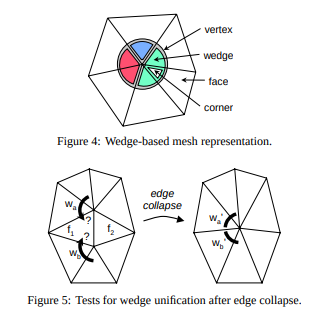
\includegraphics[width=3in]{Figures/edge_collapse.png}
    \caption{Collapsing an edge in \cite{hoppe1999new}, taking into consideration color discontinuities}
    \label{fig:edge_collapse}
\end{figure}


%%%%%%%%%%%%%%%%%%%%%%%%%%%%%%%%%%%%%%%%%%%%
\clearpage
\section{Methods}
%%%%%%%%%%%%%%%%%%%%%%%%%%%%%%%%%
\subsection{General}

The end goal of the project is to develop an efficient system for image vectorization. The system would take any image as input and output an SVG representation of the original image. The system is mainly composed of 3 different components.

%%%%%%%%%%%%%%%%%%%%%%%%%%%%%%%%%
\subsection{Sampling}

The sampling process is based on \cite{zhao2013image}. The input image is a regular bitmapped image, such as \cref{fig:arch_original}. The first step is to apply the gradient operator on the image to get the importance matrix, shown in \cref{fig:arch_importance}. This involves pixel-wise convolving with four $3\times 3$ Sobel filters (horizontal, vertical, and two diagonals) and finding the magnitude to determine the magnitude of the gradient, which is interpreted as the local information content or ``importance'' of the area surrounding a given pixel. Next, the importance matrix is thresholded so that only points of high importance are retained, shown in \cref{fig:arch_thresholded}. This is essentially a high-pass filter; low-frequency components of the image are lost. The intuition is that low-frequency elements can be represented with uniformly-colored shapes without much information loss.

Now we perform the sampling to obtain \cref{fig:arch_sampled}. The sampling density at a pixel is a function of the importance of that pixel; a higher importance leads to a higher sampling frequency. This is known as ``blue-noise'' sampling, and allows us to focus more detail on regions of higher information content. After sampling, the image is converted to a triangular mesh by performing the Delaunay triangulation, as shown in \cref{fig:arch_triangulated}.

% TODO: include formula for sampling density and explain it
% TODO: explain method for sampling (poisson disks?)

\begin{figure}[H]
    \centering
    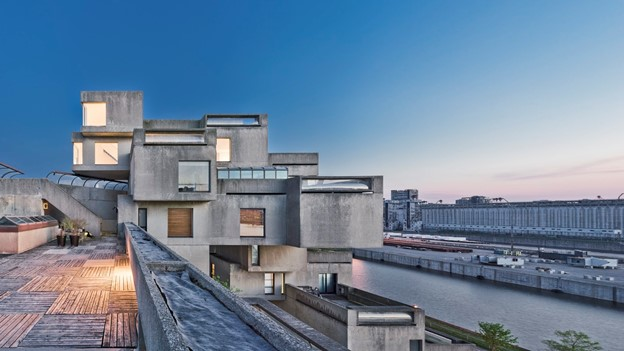
\includegraphics[width=\linewidth]{Figures/vectorization_images/original.jpg}
    \caption{Original image}
    \label{fig:arch_original}
\end{figure}

\begin{figure}[H]
    \centering
    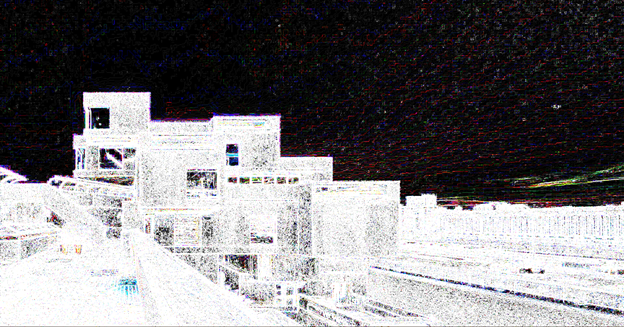
\includegraphics[width=\linewidth]{Figures/vectorization_images/importance.png}
    \caption{Importance function applied to the image}
    \label{fig:arch_importance}
\end{figure}

\begin{figure}[H]
    \centering
    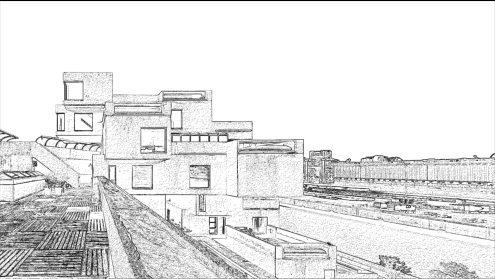
\includegraphics[width=\linewidth]{Figures/vectorization_images/thresholded.png}
    \caption{Thresholded points}
    \label{fig:arch_thresholded}
\end{figure}

\begin{figure}[H]
    \centering
    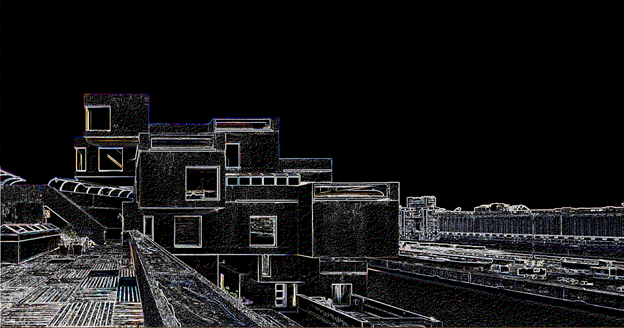
\includegraphics[width=\linewidth]{Figures/vectorization_images/sampled.png}
    \caption{Sampled points}
    \label{fig:arch_sampled}
\end{figure}

\begin{figure}[H]
    \centering
    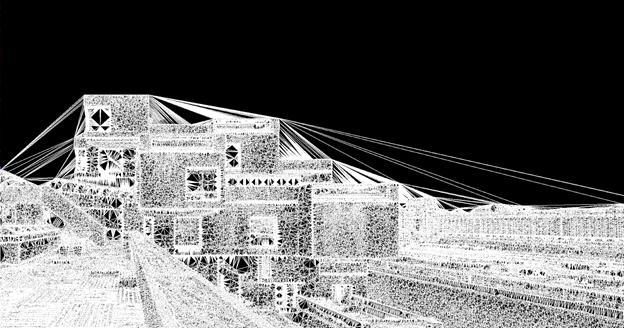
\includegraphics[width=\linewidth]{Figures/vectorization_images/triangulated.png}
    \caption{Triangulated image}
    \label{fig:arch_triangulated}
\end{figure}

%%%%%%%%%%%%%%%%%%%%%%%%%%%%%%%%%
\subsection{Mesh Optimization}

This is a future goal for spring semester and has not been implemented yet.

%%%%%%%%%%%%%%%%%%%%%%%%%%%%%%%%%
\subsection{Triangle Mesh Coloring}

We currently have three methods for determining what color to use for each triangle. The first method takes the mean of the RGB values at the three points of the triangle. The second method randomly samples a set number of integer points inside of the triangle and takes the mean of the RGB values of those points. The third method takes the mean of the RGB values at every integer point in the triangle. We note that the third method approximates the triangle, so it may sample integer points outside of the triangle. In addition, the third method utilizes the first method for small triangles, where the number of integer points inside the triangle is less than three.

%%%%%%%%%%%%%%%%%%%%%%%%%%%%%%%%%
\subsection{Writing to SVG}

We convert internal representations of triangles (tuples with 3 pairs, representing the coordinates of each point on the triangle) to an SVG file. We use Python's pycairo library to accomplish this.

In the future, we may also attempt to optimize this, such as by coding redundant information.

%%%%%%%%%%%%%%%%%%%%%%%%%%%%%%%%%
\subsection{Evaluation Metric}

We implemented an evaluation metric based on content loss from \customcite{dumoulin2017learned}. Similar to the methodology used by the authors, We use a pre-trained VGG-19 and strip off the $conv_5$ and fully-connected blocks. It is important to note that the authors used a VGG-16. We use a VGG-19, similar to \customcite{huang2017arbitrary}. In order to get the content loss between two images, we take the Euclidean distance between the outputs of the stripped VGG-19.

% We tested the content loss metric on three images related to style transfer using Generative Adversarial Networks. The images were from \url{https://www.tensorflow.org/tutorials/generative/style_transfer}. 

% \begin{figure}[H]
%     \centering
%     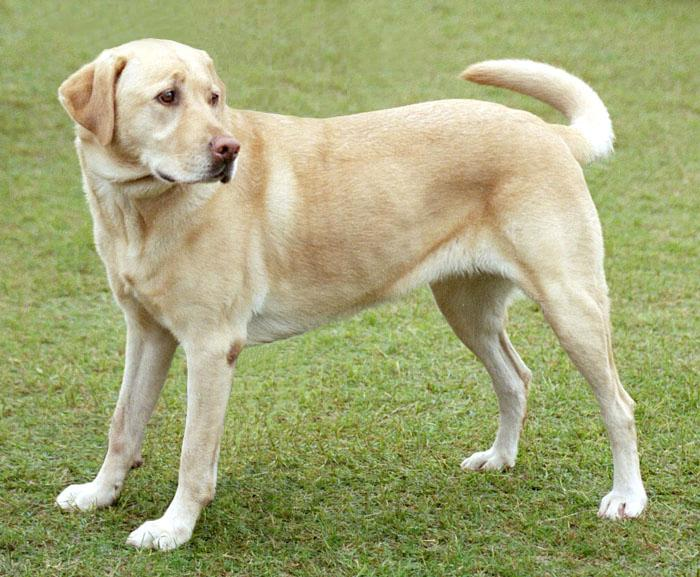
\includegraphics[width=\linewidth]{Figures/content_loss_images/lab1.jpg}
%     \caption{\href{https://commons.wikimedia.org/wiki/File:YellowLabradorLooking_new.jpg}{Yellow Labrador Looking}, from Wikimedia Commons}
%     \label{fig:lab_original}
% \end{figure}

% \begin{figure}[H]
%     \centering
%     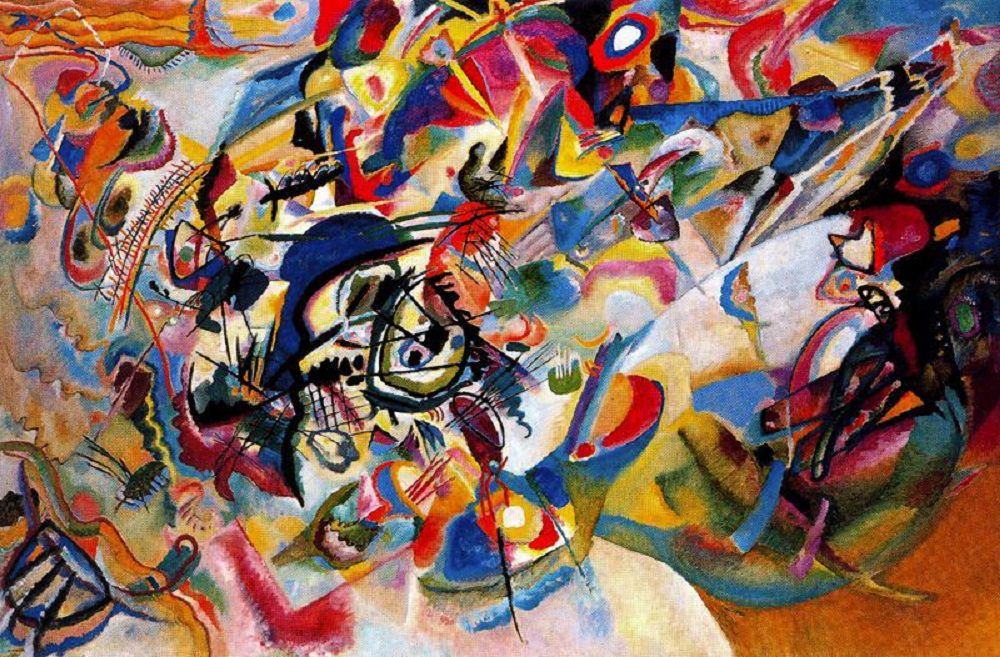
\includegraphics[width=\linewidth]{Figures/content_loss_images/lab2.jpg}
%     \caption{Composition VII by Wassily Kandinsky}
%     \label{fig:lab_style}
% \end{figure}

% \begin{figure}[H]
%     \centering
%     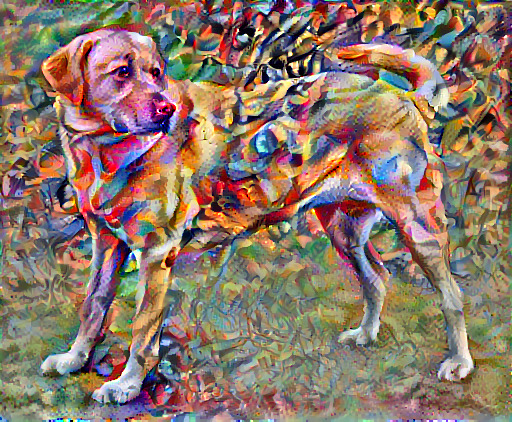
\includegraphics[width=\linewidth]{Figures/content_loss_images/lab3.jpg}
%     \caption{Generated image produced with style transfer}
%     \label{fig:lab_style_transfer}
% \end{figure}

% \cref{fig:lab_style_transfer} is generated using the content from \cref{fig:lab_original} and the style from \cref{fig:lab_style}. We calculated the content loss between all three pairings of the above images. The results are displayed in the table below.

% \begin{table}[H]
%     \centering
%     \begin{tabular}{| c | c | c |}                                             \hline
%         Image 1 & Image 2 & Content Loss                                    \\ \hline
%         \cref{fig:lab_original} & \cref{fig:lab_style_transfer} & 132352.05 \\ \hline
%         \cref{fig:lab_original} & \cref{fig:lab_style} & 190958.28          \\ \hline
%         \cref{fig:lab_style} & \cref{fig:lab_style_transfer} & 190266.86    \\ \hline
%     \end{tabular}
%     \caption{Sample content loss for example images}
%     \label{tab:lab_content_loss}
% \end{table}

% As can be seen in \cref{tab:lab_content_loss}, the lowest content loss is between \cref{fig:lab_original} and \cref{fig:lab_style_transfer}, which is expected. In addition, the content loss between \cref{fig:lab_style} and the other two images is almost the same, which makes sense, because the other two images should have the same content with different style.

% We may want to refine this evaluation metric in the future. The content loss values are extremely large and are difficult to interpret on their own. We may wish to use a baseline image when comparing the results of our project. We would thus compare three images (the original image, the vectorized image, and the baseline image). This baseline image can be arbitrarily selected. The purpose of the baseline image is to provide context to the content loss values. Similar to the above example, we would compare all three pairings of the images. We would want the content loss between the original image and the vectorized image to be the lowest. We would also want the content loss for the other two pairings (with the baseline image) to be relatively similar.

\begin{figure}[H]
    \centering
    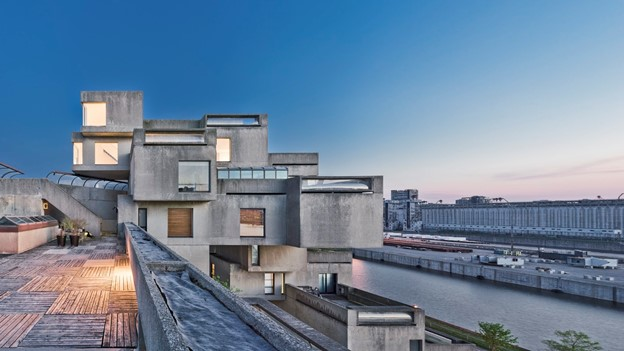
\includegraphics[width=\linewidth]{Figures/vectorization_images/original.jpg}
    \caption{Original image}
    \label{fig:house_original}
\end{figure}

\begin{figure}[H]
    \centering
    \includesvg[width=\linewidth]{Figures/vectorization_images/house_potrace.svg}
    \caption{Vectorized image created with Potrace}
    \label{fig:house_potrace}
\end{figure}

\begin{figure}[H]
    \centering
    \includesvg[width=\linewidth]{Figures/vectorization_images/house_our_method.svg}
    \caption{Vectorized image created with our method}
    \label{fig:house_our_method}
\end{figure}

\begin{table}[H]
    \centering
    \begin{tabular}{| c | c | c |}     \hline
        Method & Content Loss       \\ \hline
        Our Method & 118758.836     \\ \hline
        Potrace & 141575.78         \\ \hline
    \end{tabular}
    \caption{Content loss for vectorizing a sample image with different methods}
    \label{tab:house_content_loss}
\end{table}

As seen in \cref{tab:house_content_loss}, our method produces a significantly lower content loss than Potrace.

%%%%%%%%%%%%%%%%%%%%%%%%%%%%%%%%%
\subsection{Implementation stack}

The current implementation is a mix of Python and C++. The image processing components utilize OpenCV for GPU support and will be multi-threaded. Efficiency of the process is not a concern at this point; we care more about optimizing for the error metric. Future iterations of this project may consider efficiency of implementation.


%%%%%%%%%%%%%%%%%%%%%%%%%%%%%%%%%%%%%%%%%%%%
\clearpage
\section{Conclusion}

Image vectorization is the process of converting a raster image to a vector image, and may lead to efficiency gains for highly vectorized images. While vectorization has been used successfully on simple vector-based input images in the past such as map or typography images, we aim to improve its output on highly-geometric but less-exact images, such as architectural images. We believe that this may be useful in the architectural design process, and perhaps in other design processes whose subject is highly geometric.

We have implemented a basic framework for vectorizing raster images, primarily based on \cite{zhao2013image}. We can take an input image, perform sampling on the image, triangulate the sampled points, and produce an output image. So far we have yet to optimize this method towards architecture -- this will involve optimization stages after producing the mesh.

%%%%%%%%%%%%%%%%%%%%%%%%%%%%%%%%%%%%%%%%%%%%
\clearpage
\section{Future Work}

In the upcoming semester, we would like to experiment with different vectorization approaches. This may involve different sampling methods or different optimizations. We may choose a different method for generating vectors from the sampled points. Currently, we are using a standard Delaunay triangulation, although there may be alternative methods available.

We may change our evaluation metric if we discover a better metric. We will rank each of our approaches according to our evaluation metric. By the end of the upcoming semester, we will also produce a presentation describing our results, along with a final report that contains the final decisions made for our project.

An approximate timeline for the spring semester may look like:
\begin{description}
\item[January] Begin work on mesh optimization, review prior work.
\item[February] Continue mesh optimization, clearly define evaluation metrics.
\item[March] Begin gathering results and evaluating using given metric.
\item[April] Finish result-gathering, begin final report and presentation.
\item[May] Complete final report and presentation, present results.
\end{description}

%%%%%%%%%%%%%%%%%%%%%%%%%%%%%%%%%%%%%%%%%%%%
\clearpage
\printbibliography[
    heading=bibnumbered,
    title={References}
]

\end{document}
